\newpage

\section{Testovanie}

Cieľom overovania bolo zistiť či algoritmus na odhalovanie dlhodobých 
preferencií postavený na obdobiach dokáže poskytnúť lepšie výsledky ako 
agrgácia hodnôt.

\paragraph{Vlastné testovanie}

Preto som sa rozhodol najskôr vytvoriť jedného testovacieho požívateľa a sledovať 
ako sa s časom bude menit účinnosť obydvoch algorimtov. 

Pri tomto testovaní sa porovnával používateľov zámer z niekoľkými odporučeniami algoritmov.
Támer bol tvorený skupinov kapiel alebo typov dokumentov. Vzhľadom na unikatnosť piesni
som sa rozhodol nepoužiť pri testovani tento parameter.

Podobnosť užitočnosť odporúčaní som hodnotil podľa toho, koľko kapiel a typov dokumentu
sa nachádza aj v zámere aj vo výsledku. Tento prístup je vyjadrený matematicky 
rovnicou \ref{eq:result_set_utility}.

\begin{equation}\label{eq:result_set_utility}
užitočnosť(R) = \frac{\sum\limit_{i=0}^{N}1 + \sum\limit_{i=0}^{M} 1 +\sum\limit_{i=0}^{K}1}{3}
\end{equation}

Rovnica obsahuje \(R\) čo je množina odporúčaní, \(N\), čo je počet piesni ktoré sú aj v
zámere aj v odporúčaní, \(M\) je počet interpretov ktorý sú aj v zámere aj v odporúčaní a 
\(K\) je počet typov dokumentov ktoré su tiež prienikom odporúčaní a zámeru.

Na obrázky \ref{fig:manual_testing_results} môžeme vydieť výsledok tohoto testu.

\begin{figure}
    \begin{center}
        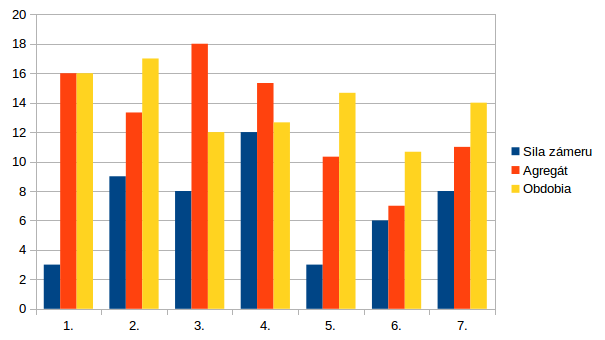
\includegraphics{manual_testing_results}
        \caption{Graf výsledkov pre manualny test}
        \label{fig:manual_testing_results}
    \end{center}
\end{figure}

Pokračovať v testoch nemalo zmysel vzhľadom na to že agregačný algoritmus v predposlednom
aj v poslednom teste vrátil rovnaké výsledky. Čo vzhľadom na jeho povahu znamená že 
menšie zámery už nemajú vpliv na jeho výsledok.

\subsection{Dotazník}

Ďaľšie testovanie prebehlo formov testovania aplikácie na webe pomocov respondentov, ktorý 
používali aplikáciu rôzne časove obdobia, následne sa im boli ponúknute odporúčania z obidvoch 
algoritmov a oni vyhodnotili ktorí im viacej vyhovuje.



